%%% "TeXing it Easy" code %%%
%%% Last modified: 16 May 2025 16:02%%%

\documentclass[letterpaper, 12pt]{article}

%%% packages
\usepackage{graphicx} % Required for inserting images
\usepackage{textcomp}
\usepackage{tipa}
\usepackage{physics}
\usepackage{fullpage}
\usepackage{amsmath, amssymb, amsthm}
\usepackage[dvipsnames]{xcolor}
\usepackage{float}
\usepackage[headheight=15pt,headsep=0.3cm,top=2.5cm, margin=2.54cm]{geometry}
\usepackage{minted}
\usepackage[backend=biber,style=apa]{biblatex}
\usepackage{lmodern}
\addbibresource{ref.bib}
\usepackage{enumitem}
\usepackage{microtype}
\usepackage{gensymb}
\usepackage{parskip}
\usepackage[normalem]{ulem}
\usepackage{hyperref}
\hypersetup{
    colorlinks=true,        % Enable colored links
    linkcolor=teal,         % Set color for internal links
    citecolor=teal,         % Set color for citations
    filecolor=teal,         % Set color for file links
    urlcolor=teal           % Set color for URLs
}

%%% header
\usepackage{fancyhdr}
\pagestyle{fancy}
\fancyhf{} % clear everything

%%% new commands
\newcommand{\define}[1]{\textcolor{blue}{\underline{#1}}} % define words
\newcommand{\cmd}[1]{\texttt{\textbackslash #1}} %write command
\newcommand{\emphasise}[1]{\textcolor{red}{\textbf{\textit{\underline{#1}}}}} % example new command
\newcommand{\mathR}{\left(0.0821 \: \frac{\mathrm{L} \cdot \mathrm{atm}}{\mathrm{mol} \cdot \mathrm{K}}
\right)} % more examples
\newcommand{\textR}{\(\displaystyle 0.0821 \: \frac{\mathrm{L} \cdot \mathrm{atm}}{\mathrm{mol} \cdot \mathrm{K}} \)} % even more examples

\begin{document}

\begin{titlepage}
    \centering
    \vspace*{2cm}
    {\Huge \bfseries \TeX ing it Easy\par}
    \vspace{2cm}
    {\Large A simple, beginner-friendly guide to \LaTeX \par}
    \vfill
    {\large October 2024--May 2025\par}
    \vspace{1cm}
    {\small Emily Zhang, Catalina Girls Who Code\par}
    \vspace{1cm}
\end{titlepage}

\tableofcontents

\fancyhf{}
\fancyhead[L]{\textsc{Contents}}
\fancyfoot[C]{\thepage}

\nocite{*}

\newpage

\section*{Preface}

\fancyhf{}
\fancyhead[L]{\textsc{Preface}}
\fancyfoot[C]{\thepage}

\addcontentsline{toc}{section}{Preface}

Hi! And hi again! Welcome to \LaTeX!

I'm beyond delighted to welcome you to \textit{\TeX ing It Easy}, a little passion project of mine, and into the realm of typesetting. This document has two objectives: 1) to help out some curious friends who want to learn to \TeX\footnote{A friend told me earlier this year that ``anything can be a verb if you try hard enough." That's my justification.} and 2) to make \LaTeX{} less intimidating.

The purpose of this document is to serve as an introduction to \LaTeX{} for anyone and everyone, including people who have never touched a computer program before. \LaTeX{} is, to put it lightly, extensive, complete with packages developed meticulously through many \TeX{} users' hard work. It's like implementing the work of a community of passionate contributors and glimpsing their expertise!

Let's begin with a story with the purpose of answering the question, ``What is the point of you doing this?''

Imagine, if you will, a seventh grader who was just introduced to the concept of making math not look like a deconstructed mess on paper. I believe in the power of a paper and pen, but on the rare occasion would be tasked with typing out math in Docs or in a text. It looks something like this:

\begin{verbatim}
x = [-b +- sqrt(b^2-4ac)]/(2a)
\end{verbatim}

When \LaTeX{} for math was introduced to me, my twelve-year-old self was not shy about asking questions. It took three people to explain the concept, and guess what? I still didn't get it. And imagine my pleasant surprise when someone told me that it's not just for pretty math; it's for pretty documents too!

One fact was easy to figure out. Helpful beginner tutorials are awfully hard to come across. Sure, there are a lot of them out there, but you have to really dig deep and figure out which ones actually suit your needs. Worse, when you're a complete beginner, you can't judge the quality of tutorials. You just have to trust every tutorial you see. As someone who is not an expert by any definition, I'm kindly requesting that you trust my tutorial, and if you're still reading, that means you do, so thank you for that!

That led to asking myself: if I were to go back in time and learn the basics of \LaTeX{} all over again, what would be my ideal tutorial? And here we are now! You've found the passion project of your friendly neighborhood beginner \TeX ie hoping to make the process easier on you than it was on me, because that's what progress is all about.

This document is a work in progress. A constant work in progress, for that matter. Always and forever, ad infinitum, until the end of time. At this point in time, though, it's considered a mostly completed work in progress, meaning I'll probably never touch it again unless you give me recommendations. Please do! If you see any discrepancies between a known fact and what's written here, do not hesitate to point them out. Same thing goes for spelling errors, grammatical errors that interfere with your understanding, etc.

Now, a clarification on the nature of \LaTeX, and more specifically on the question of whether it is a programming language or not. Some sources say yes, other say no, but in general, it's referred to as a markup language. Are markup languages programming languages? Same thing: some sources say yes, others say no. Here, we'll avoid overcomplicating it. Please keep in mind that various sources provide various answers for this question as you go through. You have complete freedom to choose which source(s) to believe (or not to believe).

Here's a bit of fair warning: \LaTeX{} is hard. Not impossible, to be sure, but hard enough to be frustrating at times. Your initial frustration is a rite of passage, and it's normal, and you'll get more comfortable the more you write. The key is practice, practice, practice.

But no need to worry! We're in this together. I'm super excited to share this with you and hope that you'll enjoy reading it as much as I enjoyed writing it.

\newpage

\fancyhead[L]{\nouppercase{\leftmark}}   % section on the left
\fancyhead[R]{\nouppercase{\rightmark}}  % subsection on the right
\fancyfoot[C]{\thepage}
\renewcommand{\sectionmark}[1]{
  \markboth{\thesection\ \textsc{#1}}{}}
\renewcommand{\subsectionmark}[1]{
  \markright{\thesubsection\ \textsc{#1}}}

\section{Introduction to \LaTeX}

\subsection{What is \LaTeX?}

Here comes the big question. What even is \LaTeX\footnote{The placement of the letters is intentional. In text, to avoid ambiguity, you would write ``LaTeX" or ``LaTex" so that it doesn't become ``latex''.}? The term gets thrown around often, especially in the academic world, but is hardly ever explained. You've likely either heard of or seen it somewhere, whether you know it or not. But what is it, really? What's with all the hype?

\LaTeX{} is, in short, a typesetting system widely used in technical writing for creating professional-looking documents. It's a standard in academia and a valuable skill to learn.

First, the pronunciation. It's not that hard to pronounce, but breaking the habit of calling it ``latex" is hard once you get used to it, so try not to get used to it! The word \TeX{} is meant to be an uppercase version of $\tau \epsilon \chi$, a Greek word meaning ``art" or ``technology", so it's pronounced ``tech" instead of ``teks." \textit{Tech}nically (wink wink), that ending is not an English sound, but as long as you're not saying ``latex'', you should be fine.

Say your first option with me: \textit{lay-tech} (IPA: /\textipa{"leItEk}/), long \emph{a}. As in you're \textit{late} to \textit{tech} because you took a super long nap and now you're frantically searching your closet for something presentable to wear and getting 10 missed calls from your stage manager.

Second option is \textit{lah-tech} (/\textipa{"lA:tEk}/), open \emph{a}. You can say the first, you can say the second, you can alternate, you can mix it up, whatever your heart desires!

Let's take a trip back to the late 1970s and talk about someone named Donald E. Knuth, the famous creator of \TeX{}. He published a multi-volume work called \textit{The Art of Computer Programming}, but when he received it, the typesetting quality was not up to standard. He set off to develop \TeX{}, an endeavour that spanned ten years. The first version of \TeX{} was released in 1982.

Another computer scientist, Leslie Lamport, came along and decided that while \TeX{} was certainly revolutionary, it wasn't as user-friendly as it could be. He built \LaTeX{} on top of \TeX{} to lift some of that precise control and make the users' lives easier.

So there's \TeX, the detailed typesetting system. Then there are word editors like Docs and Word, offering (relatively) limited control over formatting. And of course, \LaTeX, literally short for ``Lamport \TeX", striking the happy medium. Too hot? Too cold? No, just right. Cue the Disney music.

\subsection{Why use \LaTeX?}
``You could just use Google Docs." ---pretty much everyone

Yes. That is true. You could just use Google Docs and save yourself the trouble of learning a whole new skill. Why would you learn \LaTeX{}, then?

It's aesthetic. 10/10, no notes, flawlessly executed typographical perfection. And it does have practical uses! You may or may not be required to learn \LaTeX{} in college, it has become the standard in academic writing, and have you seen the gorgeous equations? Pretty \textit{and} practical---now that's a good combo.

Now to answer everyone's favorite question: which is better, typesetting or word processing? That is, \LaTeX{} or Docs?

A small warning: Some \TeX{} users feel \textit{super} strongly about it, so if any current users are reading this, remember that \textbf{this is just my opinion, not a universal truth.} My opinion is that you don't have to get married to your favorite word processor or typesetting software. In other words, it depends on what functionalities you're hoping to take advantage of.

To elaborate, Docs and Word are what's called ``What You See Is What You Get" or ``WYSIWYG" tools (isn't that so fun to say?), and \LaTeX{} and HTML are considered ``What You See Is What You Mean" or ``WYSIWYM" tools. In most ways, Docs and Word are easier, and you don't have to learn much. You just click buttons.

Word processing and typesetting are different, and each have their own time and place. Docs and \LaTeX{} aren't inherently in competition. You might enjoy using \LaTeX{} to write lab reports and papers, but find it tedious to use for grocery lists. \href{https://programmingforresearch.wordpress.com/2012/03/23/word-processor-versus-typesetter-2/}{This article} explains it nicely. While Word is great for short documents, it tends to become inefficient and annoying when dealing with long documents. On the flip side, there's no need to use \LaTeX{} when you're out shopping (but you could!).

\newpage

\section{The Basics}

\subsection{Overleaf}
The easiest \LaTeX{} editor out there to start with is Overleaf, with a user-friendly interface and resources for users of all levels of experience. All you have to do to set up Overleaf is:

\begin{enumerate}
    \item Sign up.
\end{enumerate}

That's it! The only thing you need to do is go to \href{overleaf.com}{overleaf.com} and put in your personal email.

Take a moment to get familiar with the environment. On Overleaf, most commands are just a click away, but be careful not to rely on the toolbar too much---when you start writing without the help of Overleaf, you'll need to know the commands!

At the top, there's a green ``Compile'' button, and you want to press that every so often just to make sure your code is running nice and smoothly. You also have the option to choose ``Auto-compile'' from the drop-down menu, but when you're going a bit slower, it tends to get impatient and throw errors at you. It's a race between you and the attention span of auto-compilation, and time is ticking.

If you're running your code locally, Overleaf automatically uses \texttt{pdflatex} as the engine and \TeX{} Live 2024 (as of May 2025). 

\subsection{Command syntax}
So much of \LaTeX{} depends on the humble backslash. It's completely underrated and deserves more love than it gets. Forward slash, take a backseat. We're focusing on its far less appreciated counterpart.

A nice way to get used to the syntax of any language is to look at it for a few minutes, look at the output, and see if you're able to figure it out yourself. Overleaf has great examples that you can open and look through. Once you think you've figured out some of the syntax, you might find this easier to follow.

Command syntax is fairly easy (though it may seem odd at first). \LaTeX{} commands generally look like this:

\begin{minted}[bgcolor=gray!5]{latex}
\command[optional]{mandatory}
\end{minted}
A \define{command}, as its name suggests, tells a computer to do something. Commands in \LaTeX{} are usually preceded by a backslash ($\backslash$).

A \define{parameter} is a placeholder for a value (an \define{argument}) you give to a command. For example, in this case, \texttt{optional} and \texttt{mandatory} are both parameters, but the actual values you assign to them are arguments.

There is one argument that is necessary for most commands in this format. It is, conveniently, called the mandatory argument! You need to provide a mandatory argument inside these curly brackets \{\} and optional customisations are available for some commands inside these square brackets [].

Essentially, the command tells the computer to do something, and the mandatory argument tells it what to do the command to. The optional argument adds details and customises formatting. An example is shown here:

\begin{minted}[bgcolor=gray!5]{latex}
\textbf{This is fun!}
\end{minted}
\cmd{textbf} is a simple command telling the computer to make the argument bold in the output, so it will look like:

\textbf{This is fun!}

\subsection{The document preamble}
By now you've created your file. You stare at it. A blank void stares back.

The first step is always the hardest. Before jumping into the actual typesetting piece, let's talk about the \define{preamble}.\footnote{Not the ``We the People'' kind.} The preamble is a place to style your project, similar to a CSS file linked to an HTML project.

Here's a minimal example:

\begin{minted}[bgcolor=gray!5]{latex}
\documentclass{article}
\usepackage{graphicx} % Required for inserting images
\title{Your Title Here}
\author{Your Name Here}
\date{October 2024}

\begin{document} % This is where the preamble ends

\maketitle

\section{Introduction}

\end{document}
\end{minted}
These lines are already included in a blank Overleaf document even if you didn't choose a template. If you're not using Overleaf, it might be a good idea to type these lines into your editor, customise to your liking, and follow along there.

So what do these lines mean? Let's break it down line by line:

\paragraph{Document classes} \cmd{documentclass} is a straightforward command in the preamble, and there are a few types you can choose from. \texttt{article} is pretty common and creates something like this document, \texttt{beamer} creates a slideshow presentation, and \texttt{book}, unsurprisingly, creates a book. It does take optional arguments, and \texttt{[letterpaper, 12pt]} is always my go-to set of customisations, especially since the default has insanely large margins that don't look good and doesn't optimise space while still keeping that clean, polished look. Letter paper has the dimensions we're all familiar with ($8.5 \times 11$ freedom units). % inches lol

\paragraph{Packages} Packages include additional command sequences on top of basic \LaTeX{} ones that allow for further modifications. We'll go over specific packages in detail in a later section, but whenever something says that a package is needed and you want to try it out, simply type \cmd{usepackage} somewhere in the preamble\footnote{The \texttt{hyperref} package is generally loaded last.} and the name of the mentioned package in curly brackets.

\paragraph{Header} The header will only show up if you have \cmd{maketitle} in the body. The three commands \cmd{title}, \cmd{author}, and \cmd{date} are self-explanatory. For a changing date every time you open the project, type \cmd{today} as the argument. % i call this bit "tad" since it's title-author-date but that is definitely not an official name... or is it?

Now that we've touched on the preamble, we're about to go into the body of the document! Ready? Let's do it!

\subsection{Basic formatting}

For an article-style document like this, it's most common to section using \cmd{section}, \cmd{subsection}, and \cmd{subsubsection.} If you run the following:

\begin{minted}[bgcolor=gray!5]{latex}
\section{Section 1}
\subsection*{Unnumbered Subsection}
\subsubsection{Subsubsection 1.0.1}
\paragraph{Paragraph}
\subparagraph{Subparagraph}
\end{minted}
you can see the different types of sections. Putting an asterisk * right before the argument allows you to create an unnumbered section, subsection, or subsubsection. (\cmd{paragraph} and \cmd{subparagraph} are unnumbered by default and look slightly different from sections, subsections, and subsubsections.)

Below are some examples of basic formatting:

\begin{minted}[bgcolor=gray!5]{latex}
% This is a comment. It won't show up.
This is \LaTeX{}, an \textbf{awesome} document preparation system that
lets you typeset with \textit{ease}. Isn't this font \textsl{pretty}?
Press ``enter" here $\downarrow$
and watch as the \textsc{sentence} goes on without a line break. It
doesn't
matter
how
many
times
you
try.              These spaces don't matter either.           But
press ``enter" twice, and it starts a new \textit{paragraph.} 
\emph{Add a line break}
here \\ and see the text start on a new line. Add two line breaks
\\\\ and now you have a space between paragraphs. 
\end{minted}
That will give you:

% This is a comment. It won't show up.
This is \LaTeX{}, an \textbf{awesome} document preparation system that
lets you typeset with \textit{ease}. Isn't this font \textsl{pretty}?
Press ``enter" here $\downarrow$
and watch as the \textsc{sentence} goes on without a line break. It
doesn't
matter
how
many
times
you
try.              These spaces don't matter either.           But
press ``enter" twice, and it starts a new \textit{paragraph.} 
\emph{Add a line break}
here \\ and see the text start on a new line. Add two line breaks
\\\\ and now you have a space between paragraphs. 

Notice that \cmd{emph} depends on the context it is used in. When it's used within \cmd{textit}, it undoes the italicisation, but in normal text, it italicises the argument.

\subsection{Lists, figures, tables}
Before we jump in, we've got to talk about \define{environments}!

Environments begin with \cmd{begin} and end with \cmd{end} (shocking, right?), with the argument being the name of the environment. Think of them as additions within the document with their own separate formatting, as the whole document itself is an environment: the \texttt{document} environment. Without \cmd{begin\{document\}} and \cmd{end\{document\}}, the document wouldn't even exist, defeating the purpose of us being here in the first place.

We'll keep it simple and talk about six environments here, although there are many, many more. Three of them are list environments, two of them are used to make tables, and one is for images. Starting with lists:

\subsubsection*{List environments}

There are three basic lists: \texttt{enumerate}, \texttt{itemize}, and \texttt{description.}

We begin with \texttt{enumerate}. This is a numbered list. As mentioned, we're going to start with our \cmd{begin} command and end with \cmd{end} because every beginning has an end. This is true for most things in life. Then, we'll use \cmd{item} to add items to the list.

\begin{minted}[bgcolor=gray!5]{latex}
\begin{enumerate}
    \item apples
    \item oranges
\end{enumerate}
\end{minted}
The above will give you:

\begin{enumerate}
    \item apples
    \item oranges
\end{enumerate}

Let's try \texttt{itemize}! That gives us an unnumbered list, or a bulleted list.

\begin{minted}[bgcolor=gray!5]{latex}
\begin{itemize}
    \item apples
    \item oranges
\end{itemize}
\end{minted}
we get:

\begin{itemize}
    \item apples
    \item oranges
\end{itemize}

And let's do a description list, just for the fun of it:

\begin{minted}[bgcolor=gray!5]{latex}
\begin{description}
    \item [supercalifragilisticexpialidocious] is a word that holds
    virtually no meaning but is fun to say.
    \item [strawberries] are red fruits that taste supercalifra
    gilisticexpialidocious.
\end{description}
\end{minted}
Description lists look a tiny bit different. We put the item we want to describe in the square brackets and the description outside of them.

The output:

\begin{description}
    \item [supercalifragilisticexpialidocious] is a fun word that holds virtually no meaning but is fun to say.
    \item [strawberries] are red fruits that taste supercalifragilisticexpialidocious.
\end{description}

\subsubsection*{Floats and specifiers}
Figures and table environments are \define{floats}. If you have some computer science background, you may remember floats as decimal values, but floats in this context are different.

Floats are special containers for content that can't (and shouldn't) be broken across a page. Imagine putting in an image on your document to see half of it show up on page 5 and the other half on page 6. That is, for obvious reasons, not ideal. So they kind of float around until you give them instructions on where to go.

We call those instructions on the floats \define{specifiers} because they specify where the floats should go. A combination of specifiers is often used.

\texttt{h} tells \LaTeX{} to place the float \textbf{here}, but as an approximate \texttt{t} tells it to place the float at the \textbf{top} of the page. \texttt{b} tells it to place the float at the \textbf{bottom} of the page, and \texttt{p} tells it to place the float on a special \textbf{page} for floats only.
 
\texttt{H} is a special case, one that requires the \texttt{float} package. It tells \LaTeX{} to place the float \textbf{precisely in its code location} and kind of is like an extreme version of \texttt{!h}.

\textbf{Typing \texttt{!} will override internal placement rules} that \LaTeX{} uses for determining good positions for floats. However, it won't always follow the placement that is specified to avoid the rest of the document looking like it just came out of a hydraulic press, so be mindful of that. If you used a very specific set of specifiers and it still didn't place it where you wanted it to go, it's because your document will not be pretty if the float goes there.

Here's an example combining most of the above:

\texttt{[!htbp]}

This is essentially telling \LaTeX:

\begin{enumerate}
    \item \textbf{Override} placement rules so that it is more likely to place the float where you want it.
    \item \textbf{Place the float here} or in the approximate position it is in the code.
    \item \textbf{Place the float at the top} if it can't place it there.
    \item \textbf{Place the float at the bottom} if it can't go to its code location or to the top.
    \item \textbf{Place the float on a special page for floats} if none of the above is feasible.
\end{enumerate}

As you see with this example, it's very lenient. The stricter the specifier, the harder it is for \LaTeX{} to place it there, unless you are using \texttt{H} in which case pretty much everything is overridden.

\subsubsection*{Making tables}
Below is a simple table:

\begin{minted}[bgcolor=gray!5]{latex}
\begin{table}[H]
    \centering
    \begin{tabular}{|c|c|c|}
        \hline
        \textbf{Name} & \textbf{Age} & \textbf{Favorite color} \\\hline
        Anna & 15 & red \\\hline
        Beatrice & 9 & blue \\\hline
        Caroline & 28 & green \\\hline
    \end{tabular}
    \caption{Example table.}
    \label{tab:example}
\end{table}
\end{minted}
The output is as follows:

\begin{table}[H]
    \centering
    \begin{tabular}{|c|c|c|}
        \hline
        \textbf{Name} & \textbf{Age} & \textbf{Favorite color} \\\hline
        Anna & 15 & red \\\hline
        Beatrice & 9 & blue \\\hline
        Caroline & 28 & green \\\hline
    \end{tabular}
    \caption{Example table.}
    \label{tab:example}
\end{table}

We begin by centering the table using \cmd{centering}, then opening the \texttt{tabular} environment. (\texttt{table} is a floating container that handles positioning, and \texttt{tabular} is what you use to make the table.) The \texttt{|c|c|c|} defines the structure of the table: one vertical line between each entry and two on either side. \cmd{hline} serves a similar purpose, except it creates horizontal lines instead of vertical lines.

The number of rows is flexible, but the number of columns is fixed by how many \texttt{c}s (meaning text is centered, \texttt{l} (left) or \texttt{r} (right) works too) you have. This particular table has three. That means there are three entries per row, and once you finish a row, you type \textbackslash \textbackslash{} to begin a new row.

Let's reference this table!

\begin{minted}[bgcolor=gray!5]{latex}
Table \ref{tab:example} shows the names, ages, and favorite
colors of three different people.
\end{minted}
Compiled:

Table {\hypersetup{linkcolor=black}\ref{tab:example}} shows the names, ages, and favorite
colors of three different people.

Try clicking the ``1". It's like magic the way it jumps to the table!

\subsubsection*{Inserting images}
To insert images, we'll need \cmd{usepackage\{graphicx\}} in the preamble. Assuming you're using Overleaf, upload the image and give it a name that you like. If you're not, drag the image into the same folder as the \texttt{.tex} file. 

Let's say we have an image called ``image.png". Once you upload and name the image, this places it in the document:

\begin{minted}[bgcolor=gray!5]{latex}
\begin{figure}[H]
    \centering %centers the image
    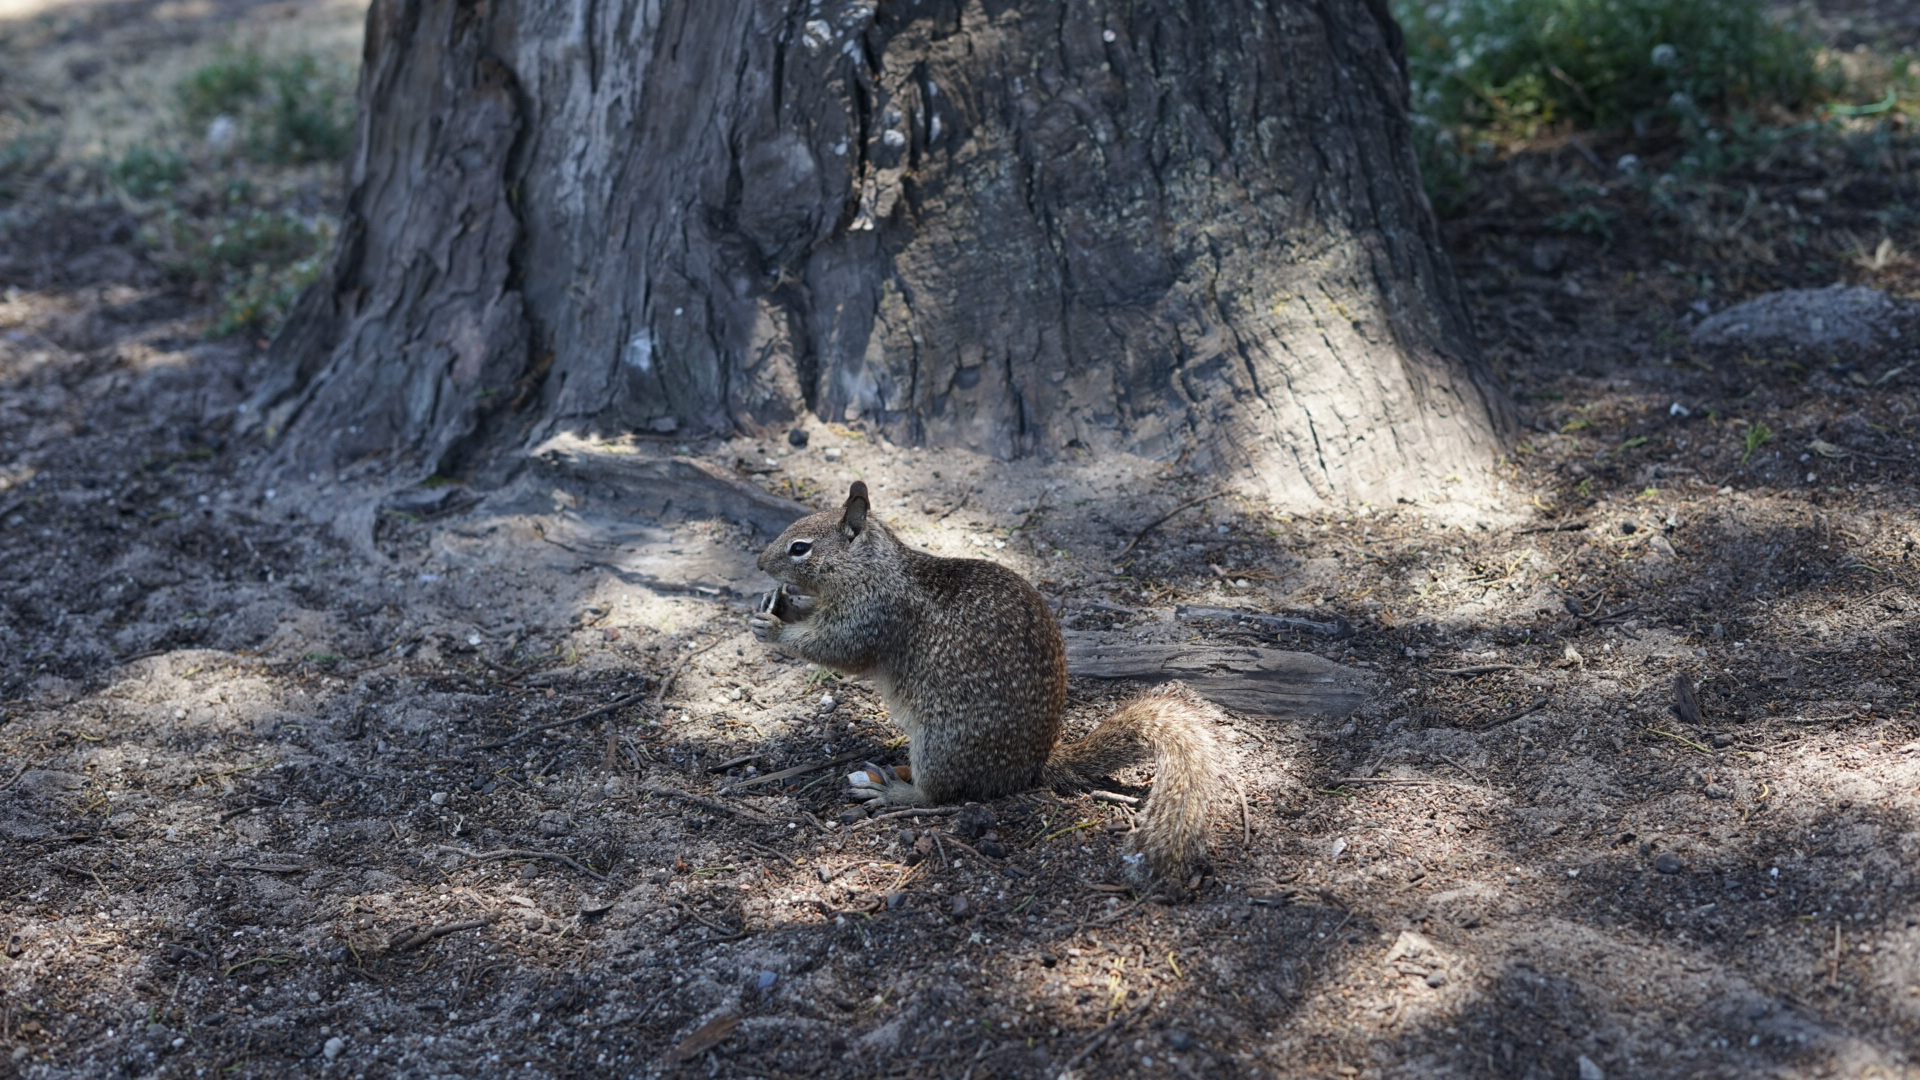
\includegraphics[width=0.5\linewidth]{image.png} %adjusts size
    \caption{Example image. Photo credits to my dad who specifically enjoys 
    photographing squirrels, for some reason?} %caption
    \label{fig:1}
\end{figure}
\end{minted}

\begin{figure}[H]
    \centering
    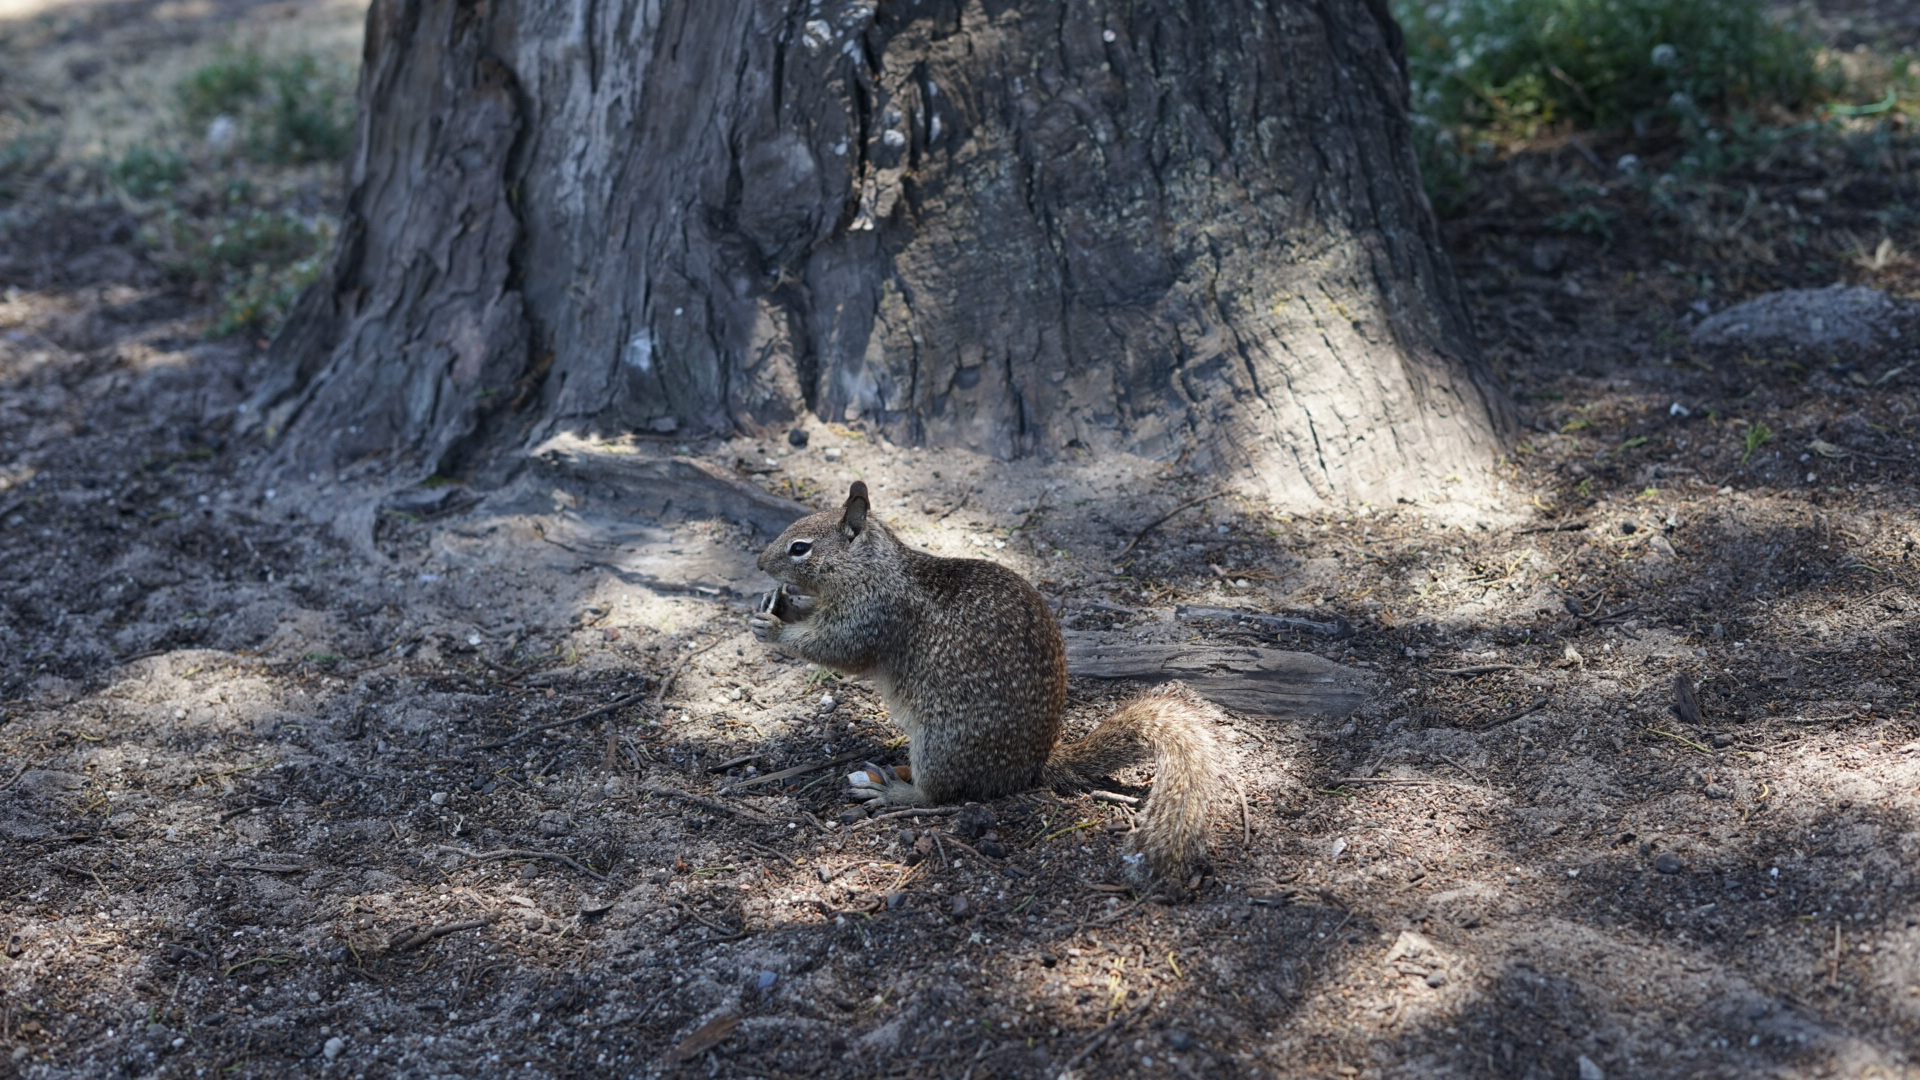
\includegraphics[width=0.5\linewidth]{image.png}
    \caption{Example image. Photo credits to my dad who specifically enjoys photographing squirrels, for some reason?}
    \label{fig:1}
\end{figure}

There's the image!

Note that \texttt{H} is used here, but you don't have to use that. Additionally, it's best to handle float placement last, after your document is mostly finalised. That way, you won't feel the need to fix the placement every few seconds.

Assume this figure is one we want to reference in the text. Besides simply saying ``see Figure 1", let's link it using \cmd{ref} as we've done with tables, like this:

\begin{minted}[bgcolor=gray!5]{latex}
Squirrels (see Figure \ref{fig:1}) are super cute.
\end{minted}
Compile that and watch it do its magic:

Squirrels (see Figure {\hypersetup{linkcolor=black}\ref{fig:1}}) are super cute.

Now you can click the little ``1" to access whichever figure you're referring to!

\subsection{Adding math}
Before anything, load the \texttt{amsmath} package. There are other packages as well, but this one is really important.

There are two primary types of math in \LaTeX: \define{inline math} and \define{display math.} Inline math is an equation that goes in the same line as the text, while display math is an equation (or series of equations) that stands alone. Here, we'll go over two examples: the Pythagorean Theorem using inline math and the quadratic formula using display math. 

Inline math is wrapped in \texttt{\$...\$} or \texttt{$\backslash$(...$\backslash$)}\footnote{\textsc{n.b.} This style is preferred for modern \LaTeX.}. To typeset the Pythagorean Theorem, type:

\begin{minted}[bgcolor=gray!5]{latex}
This is the Pythagorean Theorem. $a^2+b^2=c^2$ This is also the
Pythagorean Theorem. \(a^2+b^2=c^2\)
\end{minted}
And that gives us:

This is the Pythagorean Theorem. $a^2+b^2=c^2$ This is also the Pythagorean Theorem. \(a^2+b^2=c^2\)

Math typesetting is a skill in itself that would likely take another 30 or so pages to explain thoroughly, perhaps more. In a way, it's more intuitive---you may have seen the caret, $\wedge$, used to denote a superscript and the underscore, \_, used to denote a subscript in plain writing---but it does take time and practice to be fast at it.

To level up the complexity just by a little bit, here's the quadratic formula with display math using \texttt{\$\$...\$\$} or \texttt{$\backslash$[...$\backslash$]}:

\begin{minted}[bgcolor=gray!5]{latex}
This is the quadratic formula. \[x = \frac{-b \pm \sqrt{b^2-4ac}}{2a}\]
\end{minted}
That results in:

This is the quadratic formula. \[x = \frac{-b \pm \sqrt{b^2-4ac}}{2a}\]

Stop and admire that for a minute or two. It's gorgeous!

There are a lot of math symbols, so many that it's overwhelming to try and memorise them all. That's enough of a reason to befriend \href{https://detexify.kirelabs.org/classify.html}{Detexify}, where you can draw the symbol you want and get the command for it immediately. If you tend to forget the names of Greek letters (because, truthfully, same), this is the resource for you.

To get faster at math typesetting, try \href{texnique.xyz}{\TeX nique}! It trains you to be fast and efficient, and you can play a timed game (typing as many equations as you can within 3 minutes) or ``Zen Mode" (no time restraints).

\subsection{Symbols}

\subsubsection*{Punctuation}
Try typing this: \texttt{"It's raining," she said.}

What happens is you get two sets of right curly quotes (provided that you don't have any font packages loaded like \texttt{fontenc}).

"It's raining," she said.

Let's get some left curly quotes in here using an underrated symbol, a key that is even more underrated than the backslash: the backtick (\texttt{`}), located right under the escape button with the tilde, $\sim$. If you have the \texttt{fontenc} package loaded, you'll also need to make sure that the right quotes stay curly by using two single quotes: \texttt{''}. Otherwise, using \texttt{"} should work fine.

In other words, change it to: \texttt{``It's raining,'' she said.}

Giving us this:

``It's raining,'' she said.

Expanding on that, it's time to make up a story! A very boring story, but it'll do for now:

\begin{minted}[bgcolor=gray!5]{latex}
``It's raining,'' she said. She was so sad---she had been hoping
to go out with her friends. The storm was ill-timed, and now she was
stuck at home \dots but at least she got to read pages 17--52 of
her novel.

% left quotes: ``
% right quotes: ''
% hyphen: -
% en-dash: --
% em-dash: ---
% ellipsis: \dots
\end{minted}
That would look like:

``It's raining,'' she said. She was so sad---she had been hoping
to go out with her friends. The storm was ill-timed, and now she was
stuck at home \dots but at least she got to read pages 17--52 of
her novel.

This example contains not only the previously mentioned quotation marks, but also the hyphen (-), the en-dash (--), and the em-dash (---), as well as the ellipsis (or, colloquially, dot-dot-dot), represented by a space, a string of three dots, and another space. The ellipsis is regarded as one single character.

\subsubsection*{Special characters}

Special characters have special meanings in \LaTeX{}, so it won't take them literally if you type them on their own as you would in a word processor. Take, for example, the dollar sign: ``\$".

Try to type a dollar sign into your editor and check out what happens when you compile. An error comes up that says

\begin{verbatim}
Missing $ inserted.
\end{verbatim}

That's irritating. What if you just want a dollar sign? Simple things are so hard. You can probably guess why this error comes up: \texttt{\$} denotes math mode, so it thinks you forgot to close math mode. Luckily, there's a quick fix: escaping the special meaning with a backslash (hence why we call it an \define{escape character}). So typing:

\begin{verbatim}
\$
\end{verbatim}

will tell the computer to take the dollar sign literally.

Preceding characters with special meanings with a backslash works \dots until the special character is a backslash. Oops. How do we escape that one? Process of elimination! We can't do \texttt{\textbackslash \textbackslash}\footnote{\textsc{n.b.} Using too many manual line breaks will quickly attract underfull/overfull warnings. Consider using the \texttt{parskip} package to skip lines between paragraphs automatically. This has no connection to this topic whatsoever, but \texttt{parskip} is very helpful.}, because that's a line break. We also can't keep going down that road, because eventually the document would look like

\begin{verbatim}
\\\\\\\\\\\\\\\\\\\
\end{verbatim}

and nobody wants that. Also, it \textit{still} doesn't work.

But there is a command for this! \cmd{textbackslash} saves the day. An alternative is the \cmd{backslash} command in math mode, \texttt{\$\cmd{backslash}\$}.

Shall we wrap up our story?

\begin{minted}[bgcolor=gray!5]{latex}
``It's raining,'' she said. She was so sad---she had been hoping
to go out with her friends. The storm was ill-timed, and now she was
stuck at home \dots but at least she got to read pages 17--52 of her novel.
She downloaded \TeX{}, because that's what you do on a rainy day, but the
download  was only 50\% complete when she returned from spending \$200 
shopping online for an expensive prom dress. She wrote \textbackslash
\texttt{documentclass\{article\}} first, then started to type aimlessly.
Moral of the story: write better stories than this.
\end{minted}

``It's raining,'' she said. She was so sad---she had been hoping
to go out with her friends. The storm was ill-timed, and now she was
stuck at home \dots but at least she got to read pages 17--52 of
her novel. She downloaded \TeX{}, because that's what you do on a rainy
day, but the download  was only 50\% complete when she returned from 
spending \$200 shopping online for an expensive prom dress. She wrote
\textbackslash \texttt{documentclass\{article\}} first, then started to 
type aimlessly. Moral of the story: write better stories than this.

\newpage

\section{Diving Deeper}

\subsection{Packages!}
It's very hard to create anything that looks nice without using packages. It's possible that you could make a document look semi-decent using no packages in the preamble, but that makes your life so much harder and your document so much less interesting. \TeX{} offers a wide variety of packages, and many developers have contributed to that over the years.

In the following subsections, you're going to encounter many, many packages. When you want to test one out, simply type \cmd{usepackage} in your preamble and set the package name as the mandatory argument.

At this moment, it's worth noting that there is far more to these packages than what this document contains. However will you find out more about these packages? Documentation! Documentation! Documentation!

A quick Google search like this should help: ``CTAN package (package name)". Only searching the package name may direct you to websites that don't have to do with the package at all. Once you find the website, what you want is the documentation. There are slight (and drastic) variations between how the developers of a package choose to explain it to users, but there will be a PDF with a name like ``Package documentation" and a README file offering a brief introduction of the package's function. You can choose to read the README or to be a rebel and ignore its commanding presence.

\subsection{Customising document layout}
You've already seen the default preamble for Overleaf---it's not perfect. The margins are ridiculously huge, and all the text is squished in the center. Let me introduce you to the \texttt{geometry} package (\href{https://ctan.org/pkg/geometry?lang=en}{documentation here}).

\texttt{geometry} is incredibly flexible and is best used in tandem with other similar packages. That means that you'll be unstoppable at fulfilling whatever criteria you get for the layout of a project. Let's walk through a set of sample criteria:

``The paper should be formatted for letter-sized paper (8.5 by 11 inches) with 1-inch margins on the top, bottom, and right, and a slightly wider 1.25-inch margin on the left to allow space for binding. The font should be at 12-point size, and the text should be double-spaced throughout. Each paragraph should begin with a 0.5-inch indentation, and there should be no extra space between paragraphs."

The preamble would look like this:

\begin{minted}[bgcolor=gray!5]{latex}
\documentclass[12pt]{article} % 12pt font size

% geometry package and custom margins
\usepackage[letterpaper, top=1in, bottom=1in, left=1.25in, right=1in]
{geometry}

% setting double spacing
\usepackage{setspace}
\doublespacing

% for paragraphs
\setlength{\parindent}{0.5in} % indentation
\setlength{\parskip}{0pt}     % remove space between paragraphs

\begin{document}
Hello!
\end{document}
\end{minted}
This is only a small part of what \texttt{geometry} and other packages can do, but we'll keep it brief because it's all in the documentation.

Speaking of geometry \dots

\subsection{Adding math, the sequel}
Math part 2! Get your \texttt{amsmath} package ready, because we're going to align and number some equations.

We'll start with the simple \texttt{equation} environment.

\begin{minted}[bgcolor=gray!5]{latex}
\begin{equation} \label{eq1}
f'(x) = \lim_{h \to 0} \frac{f(x + h) - f(x)}{h}
\end{equation}
\end{minted}
That looks like:

\begin{equation} \label{eq1}
f'(x) = \lim_{h \to 0} \frac{f(x + h) - f(x)}{h}
\end{equation}

And it's numbered! You would use \cmd{ref}, as we've done before, to reference it.

Let's talk about equations with multiple parts. The ampersand (\&) in the \texttt{align} environment has a similar function to what it does for tables: it aligns wherever you place it. So writing:

\begin{minted}[bgcolor=gray!5]{latex}
\begin{align*} %the asterisk gets rid of the label
x+2y-z &= -4 \\
2x+4y-z &= 6 \\
2x+2y+3z &= 1
\end{align*}
\end{minted}
aligns the equations like so:

\begin{align*}
x+2y-z &= -4 \\
2x+4y-z &= 6 \\
2x+2y+3z &= 1
\end{align*}
where all the equals signs are in line with each other.

In this example, all of the first variables are aligned:
\begin{minted}[bgcolor=gray!5]{latex}
\begin{align*}
&x+2y-z = -4 \\
&2x+4y-z = 6 \\
&2x+2y+3z = 1
\end{align*}
\end{minted}
\begin{align*}
&x+2y-z = -4 \\
&2x+4y-z = 6 \\
&2x+2y+3z = 1
\end{align*}

That looks much better. But if you don't want any specific alignment, use the \texttt{gather} environment:

\begin{minted}[bgcolor=gray!5]{latex}
\begin{gather*}
x+2y-z = -4 \\
2x+4y-z = 6 \\
2x+2y+3z = 1
\end{gather*}
\end{minted}
\begin{gather*}
x+2y-z = -4 \\
2x+4y-z = 6 \\
2x+2y+3z = 1
\end{gather*}

Handling equations with multiple lines requires another environment. Math mode isn't great with ending a line when you reach the margin. Consider this:

\begin{minted}[bgcolor=gray!5]{latex}
\begin{equation*}
\tan^{-1}(x) = x - \frac{x^3}{3} + \frac{x^5}{5} - \frac{x^7}{7} +
\frac{x^9}{9} - \frac{x^{11}}{11} + \frac{x^{13}}{13} - \frac
{x^{15}}{15} + \frac{x^{17}}{17} - \frac{x^{19}}{19} + \frac{x
^{21}}{21} - \frac{x^{23}}{23} + \frac{x^{25}}{25} - \frac{x^{27}
}{27} + \frac{x^{29}}{29} - \frac{x^{31}}{31} + \frac{x^{33}}{33} -
\frac{x^{35}}{35} + \frac{x^{37}}{37} - \frac{x^{39}}{39} + \frac
{x^{41}}{41} - \cdots
\end{equation*}
\end{minted}
which comes out as:

\begin{equation*}
\tan^{-1}(x) = x - \frac{x^3}{3} + \frac{x^5}{5} - \frac{x^7}{7} + \frac{x^9}{9} - \frac{x^{11}}{11} + \frac{x^{13}}{13} - \frac{x^{15}}{15} + \frac{x^{17}}{17} - \frac{x^{19}}{19} + \frac{x^{21}}{21} - \frac{x^{23}}{23} + \frac{x^{25}}{25} - \frac{x^{27}}{27} + \frac{x^{29}}{29} - \frac{x^{31}}{31} + \frac{x^{33}}{33} - \frac{x^{35}}{35} + \frac{x^{37}}{37} - \frac{x^{39}}{39} + \frac{x^{41}}{41} - \cdots
\end{equation*}

and that margin destroyer is just enough to make any typesetter question their life choices. To fix this, we use \texttt{multline}:

\begin{minted}[bgcolor=gray!5]{latex}
\begin{multline*}
\tan^{-1}(x) = x - \frac{x^3}{3} + \frac{x^5}{5} - \frac{x^7}{7} +
\frac{x^9}{9} - \frac{x^{11}}{11} + \frac{x^{13}}{13} - \frac
{x^{15}}{15} + \frac{x^{17}}{17} - \frac{x^{19}}{19} + \frac{x
^{21}}{21} - \frac{x^{23}}{23} + \frac{x^{25}}{25} - \frac{x^{27}
}{27} + \frac{x^{29}}{29} \\ -
\frac{x^{31}}{31}
+ \frac{x^{33}}{33} -
\frac{x^{35}}{35} + \frac{x^{37}}{37} - \frac{x^{39}}{39} + \frac
{x^{41}}{41} - \cdots
\end{multline*}
\end{minted}
\begin{multline*}
\tan^{-1}(x) = x - \frac{x^3}{3} + \frac{x^5}{5} - \frac{x^7}{7} +
\frac{x^9}{9} - \frac{x^{11}}{11} + \frac{x^{13}}{13} - \frac
{x^{15}}{15} + \frac{x^{17}}{17} - \frac{x^{19}}{19} + \frac{x
^{21}}{21} - \frac{x^{23}}{23} + \frac{x^{25}}{25} - \frac{x^{27}
}{27} + \frac{x^{29}}{29} \\ -
\frac{x^{31}}{31}
+ \frac{x^{33}}{33} -
\frac{x^{35}}{35} + \frac{x^{37}}{37} - \frac{x^{39}}{39} + \frac
{x^{41}}{41} - \cdots
\end{multline*}

\subsection{Adding code}
Code within code within code! How does one achieve this? Let's talk about two ways to incorporate code (and, as usual, there are many more): \texttt{verbatim} and \texttt{minted}.

\texttt{verbatim} is straightforward:

\begin{minted}[bgcolor=gray!5]{latex}
\begin{verbatim}
a = 5

def greet(name):
    print("Hello " + name)

greet("World") # i have no creativity
\end{verbatim}
\end{minted}
giving us:

\begin{verbatim}
a = 5

def greet(name):
    print("Hello " + name)

greet("World") # i have no creativity
\end{verbatim}

So that works, but \texttt{minted} uses syntax highlighting, and who doesn't love colors? Take a look around the document and you'll see that all the colorful code blocks in here are formatted using \texttt{minted}. \define{Syntax highlighting} is the use of colors to  differentiate between different components of code in a particular coding language. Variable assignment might be associated with one color, while function definition might be associated with another. Here's the same example with Python with \texttt{minted}:

\begin{minted}[bgcolor=gray!5]{python}
a = 5

def greet(name):
    print("Hello " + name)

greet("World")
\end{minted}
It looks very nice with the colors, but of course not all programming languages have the same syntax. But watch as we change the language to C:

\begin{minted}[bgcolor=gray!5]{C}
a = 5

def greet(name):
    print("Hello " + name)

greet("World")
\end{minted}
This time, it doesn't recognise the Python syntax because while the code is perfectly functional in Python, we've changed the language. \texttt{minted} is really good at syntax highlighting, but it doesn't automatically recognise the language.

To use \texttt{minted}, type:

\begin{minted}[bgcolor=gray!5]{latex}
\begin{minted}{python} % or your preferred language
\end{minted}
Type your code in, and when you're done, close the \texttt{minted} environment. You only need to state the language you're using once.

\subsection{Adding a bibliography}
It's hard to overstate the importance of bibliographies. Plagiarism, despite being morally wrong, can lead to unwanted consequences, which you must have already been told many times over the years. If no one has ever held up a big sign in front of you or given you a huge presentation telling you ``PLAGIARISM IS BAD!", then kindly allow me to be the first---

{\Large PLAGIARISM IS BAD!}

In some ways, doing citations is a lot like doing your taxes. They're bewildering at first, and if you don't do them right, you get in trouble. To streamline the process of typing out each citation by hand, there are bibliographic managers available to use, such as Zotero and Mendeley.

There are multiple ways to create a bibliography, one of them being the \texttt{biblatex} package. Load this package with the \texttt{biber} backend (in the preamble) like so:

\begin{minted}[bgcolor=gray!5]{latex}
\usepackage[backend = biber, style = apa]{biblatex}
\end{minted}
The citation style can be changed according to your preferences. Now we need to make a \texttt{.bib} file, where all the citations are stored. In Overleaf, add a new file by clicking on the file button on the top left, give it a name, and change the extension to .bib. We'll use \cmd{addbibresource} to specify where the citations should come from. A file called ``ref.bib", for example, would be referenced like this:

\begin{minted}[bgcolor=gray!5]{latex}
\addbibresource{ref.bib}
\end{minted}
The .bib file is empty at the beginning, so we need to create some entries. (This is in the .bib file, not in the .tex.) An entry looks something like this:
\begin{minted}[bgcolor=gray!5]{bibtex}
@book{knuth1983texbook,
  author    = {Knuth, Donald E.},
  title     = {The \TeX book},
  edition   = {2nd},
  publisher = {Addison-Wesley},
  year      = {1983},
}
\end{minted}
Now that we've created an entry, we'll put it into the text!\footnote{\textsc{n.b.} You need an in-text citation for the full citation to show up in the ``References" section; otherwise, nothing will happen. Add \cmd{nocite\{*\}} in the body to remove this requirement.}

\begin{minted}[bgcolor=gray!5]{latex}
This is a sentence containing a citation \parencite{knuth1983texbook}.
\end{minted}
Once you compile, you'll see that two things happen. The first is the addition of a citation to the end of your sentence:

This is a sentence containing a citation \parencite{knuth1983texbook}.

Secondly, a ``References" section is added at the very end with a citation that looks like this:

Knuth, D. E. (1983). \textit{The \TeX book} (2nd). Addison-Wesley.

When you click on your in-text citation, it automatically takes you to the references section where the full citation is located.

\subsection{Creating your own commands}
Creating your own commands has a function (pun maybe intended) similar to that of creating functions in other languages. Take this, for example:

\begin{minted}[bgcolor=gray!5]{latex}
\textcolor{red}{\textbf{\textit{\underline{A compelling point.}}}}
\end{minted}
That gives you:

\textcolor{red}{\textbf{\textit{\underline{A compelling point.}}}}

Seems like a good way to highlight a compelling point \dots if it weren't so tedious. The braces are easy to get lost in. By creating a new command, we only have to type it out once. The command for making new commands is, you guessed it, \cmd{newcommand}.

We start with \cmd{newcommand}, then name the command. The name can't be the same as an existing command. Here, we call it \cmd{emphasise}. Then in the square braces, we define the number of arguments it takes. This command takes one. We end by defining what the command should do to the argument just like defining a function.

In the preamble, let's try:

\begin{minted}[bgcolor=gray!5]{latex}
\newcommand{\emphasise}[1]{\textcolor{red}{\textbf{\textit{\underline{#1}
}}}}
\end{minted}
And now in the body:

\begin{minted}[bgcolor=gray!5]{latex}
\emphasise{Another compelling point.}
\end{minted}
Which gives you:

\emphasise{Another compelling point.}

Looking at this command in action:

\begin{minted}[bgcolor=gray!5]{latex}
Here's some text. \emphasise{A compelling point!} Here's some more
text. \emphasise{Something interesting.}

Here's some text. \textcolor{red}{\textbf{\textit{\underline{A 
compelling point!}}}} Here's some more text.
\textcolor{red}{\textbf{\textit{\underline{Something interesting.}}}}
\end{minted}
Here's some text. \emphasise{A compelling point!} Here's some more
text. \emphasise{Something interesting.}

Here's some text. \textcolor{red}{\textbf{\textit{\underline{A 
compelling point!}}}} Here's some more text.
\textcolor{red}{\textbf{\textit{\underline{Something interesting.}}}}

Look how much more efficient the first one is! This is why defining
custom commands are useful.

Nice! We've done it! We've defined a command that takes one argument, and you can easily expand it to take two, or three, or more. Now what about a command that doesn't take any arguments?

Let's say you're in chemistry class and you want to typeset the ideal gas constant, $R$. You'd type:

\begin{minted}[bgcolor=gray!5]{latex}
\[\left(0.0821 \: \frac{\mathrm{L} \cdot \mathrm{atm}}{\mathrm{mol} \cdot
\mathrm{K}}\right)\]
\end{minted}
Which comes out to be:

\[0.0821 \: \frac{\mathrm{L} \cdot \mathrm{atm}}{\mathrm{mol} \cdot \mathrm{K}}\]

and that looks fine. But you probably don't want to type that out every single time. Here, we'll omit the optional argument and go straight into defining our command after naming it.

\begin{minted}[bgcolor=gray!5]{latex}
% You may find it helpful to define two versions of the command, one that
% is used in math mode and one that is used in line with the text. 
% You can also wrap your code in \ensuremath for this, but since this 
% code is nice and functional it's probably not a good idea to risk 
% breaking it!
\newcommand{\mathR}{\left(0.0821 \: \frac{\mathrm{L} \cdot \mathrm{atm}}
{\mathrm{mol} \cdot \mathrm{K}} \right)}
\newcommand{\textR}{\(\displaystyle 0.0821 \: \frac{\mathrm{L} \cdot
\mathrm{atm}}{\mathrm{mol} \cdot \mathrm{K}} \)}

\begin{document}

The ideal gas constant, \textR, is used in the formula $PV = nRT$.

$$(0.986 \: \mathrm{atm})(1 \: \mathrm{L}) = \mathR (293\mathrm{K})(n)$$
$$n = 0.041 \: \mathrm{mol}$$

Now compare that to this:

$$(0.986 \: \mathrm{atm})(1 \: \mathrm{L}) = \left(0.0821 \: \frac{
\mathrm{L} \cdot \mathrm{atm}}{\mathrm{mol} \cdot \mathrm{K}} \right) 
(293\mathrm{K})(n)$$
$$n = 0.041 \: \mathrm{mol}$$

\end{document}
\end{minted}
And that gives you:

The ideal gas constant, \textR, is used in the formula $PV = nRT$.

$$(0.986 \: \mathrm{atm})(1 \: \mathrm{L}) = \mathR (293\mathrm{K})(n)$$
$$n = 0.041 \: \mathrm{mol}$$

Now compare that to this:

$$(0.986 \: \mathrm{atm})(1 \: \mathrm{L}) = \left(0.0821 \: \frac{
\mathrm{L} \cdot \mathrm{atm}}{\mathrm{mol} \cdot \mathrm{K}} \right) 
(293\mathrm{K})(n)$$
$$n = 0.041 \: \mathrm{mol}$$ % OK WAIT THIS ACTUALLY WORKED!??!?!?! IM JUMPING FOR JOYYY

Same exact equation, but a whole lot more work. You get the point: custom commands are readable, efficient, and save you from having to do all of that unnecessary work, especially when you're using the macro multiple times. This is where it really gets exciting, because you can create commands that are much more complicated than these examples. The sky's the limit! (Or maybe 12 seconds of compile time is the limit. Is that what it is on Overleaf?)

\subsection{Embedding links}
For this, we'll need the \texttt{hyperref} package. Embedding links is super simple, and it looks like this:

\begin{minted}[bgcolor=gray!5]{latex}
This is an entertaining \href{https://www.youtube.com/watch?v=yKQ_sQKBASM}
{video}.
\end{minted}
Giving you:

This is an entertaining \href{https://www.youtube.com/watch?v=yKQ_sQKBASM}
{\textcolor{black}{video}}.

When you click ``video", the link will come up, but it's sneaky because it's the same color as the rest of the text. Unlike Docs, it won't make it clear to you that it's a link unless you tell it to. To change the color, add the following to your preamble:

\begin{minted}[bgcolor=gray!5]{latex}
\usepackage[dvipsnames]{xcolor} %for more color options
\hypersetup{
    colorlinks=true,
    urlcolor=<color>
}
\end{minted}
and pick any color from the list. (See \href{https://www.overleaf.com/learn/latex/Using_colors_in_LaTeX}{Using colors in LaTeX.})

\subsection{Changing the font}
What?! Why would you even be here? This was a test! You don't like Computer Modern?

Just kidding \dots maybe. You can absolutely change the font, and in some cases it's essential to pick the right font. Here's an in-depth \href{https://designmodo.com/font-psychology/}{article} on font psychology and a quick overview on how to switch between fonts.

Let's pick an aesthetic one. \texttt{tgschola} is pretty. In the preamble, add:

\begin{minted}[bgcolor=gray!5]{latex}
% Another package for fonts, `fontspec`, cannot be used with
% pdflatex.
\usepackage[T1]{fontenc}
\usepackage{tgschola}
\end{minted}
if you want the entire document to be in {\fontfamily{qcs}\selectfont this font.
}

{\fontfamily{ppl}\selectfont Switching between fonts
} {\fontfamily{bch}\selectfont is nice and easy
} {\fontfamily{qag}\selectfont in the body of the document.
} To switch fonts for only a section of text, add the font code (\textit{not} the package name) into this command:

\begin{minted}[bgcolor=gray!5]{latex}
% `qcs` is the font code for the font `tgschola`.
{\fontfamily{qcs}\selectfont Here's some text in the \texttt{tgschola} 
font.} Here's some text in Computer Modern.
\end{minted}
The output:

{\fontfamily{qcs}\selectfont Here's some text in the \texttt{tgschola} font.} Here's some text in Computer Modern.

Overleaf's \href{https://www.overleaf.com/learn/latex/Font_typefaces}{reference guide} for fonts contain the names and codes of fonts.

\newpage

\section{Additional Resources}

\subsection{Local editing}

The time has come for you to find a local (in your computer, not online) editor to trust your files with\footnote{See \href{https://tex.stackexchange.com/questions/193810/online-latex-editor-or-local-latex-editor}{``Online LaTeX editor or local LaTeX editor?''.}}. If you want to make longer, more complicated documents without having to pay, you can \href{https://www.latex-project.org/get/}{get a full distribution of \LaTeX{} here} for your device. You can find most things you'll need on \href{https://ctan.org/?lang=en}{CTAN}, the Comprehensive \TeX{} Archive Network that contains all things \TeX. Having a local setup installed just in case something tragic like a power outage happens is generally a good safety measure. With the amount of power outages that happen during finals season (why are power outages always during midterms?!), it's probably something you want to do, especially if you type up your notes digitally or have review sheets.

But let's take a pause and go over how to actually install the distribution you want \dots with some links! Here is \href{https://miktex.org/howto/install-miktex}{how to install MiK\TeX} (Windows) and \href{https://www.tug.org/mactex/mactex-download.html}{how to install Mac\TeX} (macOS). These two sites should walk you through the steps. Once you have that installed, find and install an editor\footnote{\textsc{n.b.} A really common mistake is having an editor installed but not having \TeX{} installed. Make sure you have both!} that you like.

You will, regrettably, find out that you've been taking too much of Overleaf for granted once you transition from online editing to local editing, but with the right approach, it's manageable. So here are some tips:

\begin{itemize}
\item \textbf{Know your terminal.} Get well acquainted with terminal commands and don't be scared of them!\footnote{Except \texttt{sudo rm -rf /}. Don't run that one just because you want to see what happens---look it up first.} It looks like a random appendage with no practical uses, but your terminal is your friend.
\item \textbf{Compile frequently.} Some editors don't have that side-by-side view like Overleaf does, and they certainly don't have auto-compile\footnote{MY LOVE.}, so it's easier for errors to slip past you without you noticing.
\item \textbf{Organise your files.} Organisation is key, especially when you want to quickly find a file. 
\item \textbf{Back up your work regularly.} Git (\ref{git}) is perfect for this.
\end{itemize}

All of this sounds quite tedious, but it can actually be really beneficial to edit locally. You're not dependent on the internet (so you can \TeX{} away peacefully while the power's out), it runs faster than Overleaf, and it teaches you a lot about how your computer works. Not to mention Overleaf can change its pricing and policies at any time, and if the platform goes down, your projects go down with it. We still love Overleaf, though, with all its articulate \href{https://www.overleaf.com/learn}{documentation}.

\subsection{The art of question asking}

\subsubsection*{Building your question}

There are no bad questions; only poorly phrased questions. Asking a good question takes a bit more time and effort than just throwing your ideas out there, but the rewards far outweigh the risks. The general components of a (good) question are the following:

\begin{enumerate}
\item \textbf{Title/subject line.} Counterintuitively, you may have some trouble getting help if the first line they see is: ``HELP!!!!!!!!!!!!!!!" Or something vague like: ``Can you help me with LaTeX?" You'd be much more likely to receive a useful answer with a more specific title. An example could be: ``Error with \texttt{align} environment in LaTeX for multiline equations".
\item \textbf{The research you've done and what you've tried already to solve the problem.} This shows that you've put in the work to try to solve your own problem before asking for help and makes the whole troubleshooting process far more efficient.
\item \textbf{A minimal, reproducible example.} More on this later, but this is essentially a self-contained snippet of code.
\item \textbf{Relevant error messages.} It's best to copy error messages verbatim, because errors are known to be a bit cryptic, and what you think it means isn't always what it actually means. 
\item \textbf{Formalities.} Never compromise courtesy for the sake of succinctness! Be kind and thoughtful in your phrasing, and keep an open mind.
\end{enumerate}

\subsubsection*{Minimal reproducible examples}
Jump for joy, everyone! We're talking about MREs!

A \define{minimal reproducible example (MRE)} (also known as a \textit{minimal workable example (MWE)} and \textit{reprex}, among other names\footnote{Some people define these terms separately and some use them interchangeably.}) is a bit of source code that demonstrates a problem that you have/how something should work and is able to be replicated.

Word by word, this means:

\paragraph{Minimal} Sending minimal examples helps to avoid unnecessary distractions that don't affect your code and could be mistakenly considered part of it. Identifying the core issue is easiest when it doesn't come with a 60-page document.

\paragraph{Reproducible} \define{Reproducibility}, in a broad sense, refers to whether someone else can repeat what you've done and obtain the same results. From a coding perspective, code is reproducible when someone else running the code gets the same output, ensuring smooth collaboration, facilitating consistent troubleshooting, and confirming the validity of your work.

\paragraph{Example} An example. No special definition. Just what it sounds like.

Making MREs, like all else in \LaTeX, takes practice, and StackOverflow has a wonderfully helpful \href{https://stackoverflow.com/help/minimal-reproducible-example}{guide} to creating an MRE.

When you're done with your MRE, insert it as code by using a code block. Several online fora support Markdown syntax for this. Markdown is a lightweight markup language that works in a way similar to \LaTeX{} (but is thankfully much easier, to save some time and tears). Here's an example:

\begin{minted}[bgcolor=gray!5]{markdown}
An example question. How do I do abc?

This is my code:

```latex
\textbf{Here is a code block.}
$a^2+b^2=c^2$
```

But it gives me this error:

> This is an example error message. We call it a blockquote.

This is inline `code` in a monospace font.

I've already tried: 
- **A bold list item.**
- *An italic list item.*
- _Another italic list item._
\end{minted}
Last but certainly not least: \textbf{Don't send screenshot MREs!!!!} Always send them in text so that they're easy to copy and paste.

\subsection{Sharing and collaborating}
\label{git}

\subsubsection*{Git, a version control system}
There's a joke that says the creator of Git, Linus Torvalds, named it that because he doesn't understand semantics. While that's amusing, it couldn't be further from the truth. The versatility of ``git'' contributes to its charm. Let's attempt to git gud at Git!

This \href{https://docs.github.com/en/get-started/learning-about-github/github-glossary}{glossary} helps you learn the vocabulary that comes with GitHub, an online platform that hosts Git repositories. But because this list is thorough, some terms are mixed in there that aren't necessarily super helpful for getting started with, so we'll just go over the basic terms.

A \define{repository} holds your project with relevant files. There's your \define{remote repository} (hosted on the internet) and your \define{local repository} (inside your computer). 

A \define{branch} is a contained version of your project where you can safely experiment without disturbing your main branch. Typically, when you work with others, you'll request to merge your branch into the main branch through a \define{pull request} on the web.

The first thing you'll need to do is create a repository. You can choose whether to initiate the repository with a README that is used to describe the project. To work on your repository locally, clone it to your computer by typing this terminal\footnote{May differ with Windows.} command with its URL:

\begin{verbatim}
git clone <url>
\end{verbatim}
Let's go through an example workflow!\footnote{See a \href{https://www.atlassian.com/git/tutorials/comparing-workflows}{comparison of Git workflows} here.} Assume your directory is

\begin{verbatim}
/Users/SusieQ/Documents/finalproject/
\end{verbatim}
and you already have a remote (on GitHub or a similar platform) version synced to your local copy.

Your terminal is ready to do some cool work. Start by changing the directory:

\begin{verbatim}
cd /Users/SusieQ/Documents/finalproject/
\end{verbatim}
then move onto a simple

\begin{verbatim}
git pull
\end{verbatim}
to make sure that the remote and local repositories are the same. If they are, your terminal should show

\begin{verbatim}
Already up to date.
\end{verbatim}

Amazing! Now let's get a separate branch. Type:

\begin{verbatim}
git checkout -b branch-name
\end{verbatim}
to make a new branch. This is where you'll be committing before you merge the branch with \texttt{main}\footnote{\texttt{main} used to be called \texttt{master} before they changed it.}.

Set the upstream after you've created a new local branch. You only need to do this once, the first time you push a new branch that doesn't already exist on the remote. Running this command will track the local branch with the remote branch of the same name on \texttt{origin}, which is the default name of the remote repo. (Git prompts you to do this if you forget.)

\begin{verbatim}
git push --set-upstream origin branch-name
\end{verbatim}
After everything is set: stage, commit, push, merge! It doesn't rhyme. But say it a few times and it'll start sounding catchy. Or not. Use:

\begin{verbatim}
git add .
\end{verbatim}
to stage all of your changes. Commit the changes with a \textit{clear} message:

\begin{verbatim}
git commit -m "whatever you did, short and sweet"
\end{verbatim}
and push them:

\begin{verbatim}
git push origin branch-name
\end{verbatim}

When you've made all the edits you want on that branch, you'll be ready to merge them into your main branch. Type: 

\begin{verbatim}
git checkout main
\end{verbatim}
to switch to the main branch. Here's where you pray that you have no conflicts. Cross your fingers, knock on wood, do all the things. Conflicts happen when changes are ``competing'' with each other, such as when one person edits part of a file and another person makes different edits on the same part.

For now, look on the bright side and assume there are no conflicts. You should be able to merge changes from \texttt{branch-name} with:

\begin{verbatim}
git merge branch-name
\end{verbatim}
and once you've done this, your \texttt{main} branch will be updated.\footnote{Run \texttt{git pull} before this when working with others.}

\subsubsection*{Pastebins}
Pastebins are a lot better for sharing smaller snippets of temporary code instead of big projects. You don't need software like Git to use a pastebin because they're generally web-based.

A popular pastebin is called \dots wait for it \dots wait for it \dots \href{https://pastebin.com/}{Pastebin}! It's as simple as making a new paste, choosing the syntax highlighting you need, then saving it. Pastebins are public by default but there is an option to make them private when you're configuring the paste.

\subsection{10 golden rules of \TeX}
\begin{enumerate}
\item Never write $sin(\theta)$ or $cos(\theta)$. We write $\sin(\theta)$ and $\cos(\theta)$. ($\displaystyle{\frac{dy}{dx}}$ and $\displaystyle{\dv{y}{x}}$ are still up for debate, though.)

\item Be kind to the software and to yourself. Try not to force \LaTeX{} to do something it doesn't want to do.

\item Practice. Practice more. Practice even more. At the very beginning, \LaTeX{} was \textit{not} my friend. It likes to scare you and make you think that even the smallest errors are catastrophic. But they are not! The more you practice, the faster you will become. Bringing us to:

\item Trust yourself over the error messages. Use the console as a guide, not a textbook, and fix errors in the way that you know how. One small error can sometimes trigger a cascade of unrelated messages. If you can identify the root of the problem, by all means, fix it with confidence.

\item Embrace the canon events! Some of these include:

\begin{itemize}
\item Doing something the long way. Learning the easy way too late. Still doing it the long way because it's become a habit.
\item Hearing ``just use Docs'' or ``just use Word'' for the 109238103851032599th time.
\item Watching your console losing its mind when you've only dropped a single bracket.
\item Overfull hbox (badness 10000).
\end{itemize}

\item If it compiles, it works. No further questions.\footnote{Sadly, this is not true. You should take time to fix errors/warnings!}

\item Try to avoid forcing things. The momentary relief may manifest itself into bigger problems.

\item Live laugh love autocompile.

\item If someone dares to disrespect the name of \LaTeX{} (i.e. by calling it ``latex''), you are henceforth obligated to answer, in the most obnoxious voice possible, ``Erm, actually, it's pronounced (insert your favorite pronunciation here).''

And remember, the most important of all: 

\item Never ever give in to the allurements of WYSIWYG editors. You are a certified \TeX ie and proud of it. Even if it decides to go against your wishes. 

\end{enumerate}

\subsection{Further reading}
\href{https://tex.stackexchange.com/help/how-to-ask}{How do I ask a good question?} \\
\href{https://www.overleaf.com/learn/latex/Free_online_introduction_to_LaTeX_(part_1)}{Introduction to \LaTeX} \\
\href{https://www.overleaf.com/learn/latex/Learn_LaTeX_in_30_minutes}{Learn \LaTeX{} in 30 minutes} \\
\href{https://www.learnlatex.org/}{Learn\LaTeX.org} \\
\href{https://www.cmor-faculty.rice.edu/~heinken/latex/symbols.pdf}{List of mathematical symbols} \\
\href{https://www.latex-project.org/}{\LaTeX -- A document preparation system}
\\
\href{https://visualmatheditor.equatheque.net/doc/texbook.pdf}{The \TeX book}\footnote{\TeX{} is not exactly the same as \LaTeX{}, but it's a good read nonetheless.}

\newpage

\section*{Conclusion and acknowledgments}

\fancyhf{}
\fancyhead[L]{\textsc{Conclusion and acknowledgments}}
\fancyfoot[C]{\thepage}

\addcontentsline{toc}{section}{Conclusion}
\textsc{Oh my days we actually did it.} It's happening! We're done!

\sout{Chat, what the sigma? We fanum taxed the whole document? We're so skibidi!} \footnote{??? Who said that? (That was for a very specific member of our Girls Who Code community.)}

The evolution of this document from a scramble of random notes to this is absolutely insane, and I'm so excited to see where we go next! It started out as bullet points that were hardly connected to each other, then became a short and simple guide of more bullet points that were somewhat connected, then, finally, 30+ pages of silliness and technicality.

This is just a fraction, a tiny, tiny fraction, of what there is to know about \LaTeX. It's a conclusion of an introduction, the end of a beginning. (Commencement address moment.) There will always be more to learn, but for now, enjoy your new \TeX{} knowledge---this language truly is remarkable.

Thank you to Mrs. Mulgrew for always being a wonderful mentor and my biggest cheerleader in the midst of navigating \LaTeX. Thank you to my friends, whose struggles with Docs never doing equations right inspired me to share my learning experience. Thank you to my teachers, whom I completely accidentally overheard talking about how hard it is to use Word, for the same reason.

Thank you, too! Yes, you, the lovely reader of this document who indulged in my passion, because without you I'd just be talking to the void. And that's embarrassing.

And if there's one thing I've learned throughout these months of searching and writing, it's that investing your time into an idea, even if you think it's a silly little idea that won't take you anywhere and even if it doesn't actually take you anywhere, is never a waste. Go do that thing you've always wanted to do! This is your sign!

Please \href{https://github.com/leucinemymind}{find me on GitHub} to share any proposed edits---your feedback is much appreciated! Again, thank you so so much for reading my glorified rant. This was fun!

All the best,

Emily
\newpage

\printbibliography[heading=bibintoc, title={Citations}]

\fancyhf{}
\fancyhead[L]{\textsc{Citations}}
\fancyfoot[C]{\thepage}

\end{document}
